% =========================================================================== %
% Yes. This is a document.

\documentclass[
	english,
	aspectratio=169,
	table
]{beamer}

% =========================================================================== %
% Theme
\usepackage{scrlfile}
	\ReplacePackage{beamerthemeSHUR}{./sty/beamerthemeSHUR}
	\ReplacePackage{beamerinnerthemefancy}{./sty/beamerinnerthemefancy}
	\ReplacePackage{beamerouterthemedecolines}{./sty/beamerouterthemedecolines}
	\ReplacePackage{beamercolorthemechameleon}{./sty/beamercolorthemechameleon}

\usetheme[
	pageofpages=/,
	bullet=circle,
	titleline=true,
	alternativetitlepage=true,
	watermark="",
	watermarkheight=0px,
	watermarkheightmult=0
	]
{SHUR}

% =========================================================================== %
% the usual stuff

\usepackage[utf8]{inputenc}
\usepackage[T1]{fontenc}
\usepackage{babel}
\usepackage{lmodern}
\usepackage{microtype}
\usepackage{csquotes}
\usepackage{xspace}

\usepackage{tabularx}
\usepackage{booktabs}
\usepackage{multirow}

\usepackage{color, colortbl}
\usepackage{xcolor}
	\definecolor{tabhighlight}{RGB}{230,240,255}

\usepackage{tabto}

\usepackage{minted}
	\usemintedstyle{friendly}

\usepackage{tikz}
	\usetikzlibrary{positioning}
	\usetikzlibrary{matrix}
	\usetikzlibrary{shapes.geometric}
	\usetikzlibrary{backgrounds}
	\usetikzlibrary{calc}
	\usetikzlibrary{decorations.pathreplacing}
	\tikzstyle{every picture}+=[remember picture] 
\usepackage{adjustbox}

\usepackage{amsmath}
\usepackage{physics}

\usepackage[most]{tcolorbox}
	\tcbsetforeverylayer
		{colback=cyan!10!white,
		 colframe=cyan!75!black,
		 arc=0pt,
		 outer arc=0pt
		}
	\newtcolorbox{codebox}[1][Code]
		{colback=black!5!white,
		 colframe=blue!40!black,
		 title=#1,
		 leftupper=6mm
		}
	\newtcolorbox{cmdbox}[1][Command Line]
		{colback=black,
		 coltext=white,
		 fontupper=\ttfamily ,
		 colframe=blue!40!black,
		 title=#1,
		 outer arc=0pt
		}
	\newtcolorbox{warnbox}[1][Warning]
		{colback=black!5!white,
		 colframe=red!40!black,
		 title=#1
		}
	\newtcolorbox{hintbox}[1][Hint]
		{colback=black!5!white,
		 colframe=green!40!black,
		 title=#1
		}
	\newtcolorbox{defbox}[1][Code]
		{colback=cyan!10!white,
		 colframe=cyan!90!black,
		 title=#1
		}
	\newtcolorbox{recapbox}[1][Code]
		{colback=yellow!10!white,
		 colframe=yellow!90!black,
		 coltitle=black,
		 title=#1
		}
%==============================================================================%
% GLOBAL MACROS

\newcommand*{\zB}{e.\,g. }
\newcommand*{\ie}{i.\,e. }

\newcommand{\Thus}{\ensuremath{\Rightarrow}\xspace}
\newcommand{\thus}{\ensuremath{\rightarrow}\xspace}

\newcommand*{\tabcrlf}{\\ \midrule}			% actually still allows for optional argument

\newcommand*{\inPy}[1]{\mintinline{python}{#1}}

\newcommand*{\todo}[1]{{\color{red}TODO: #1}}
\newcommand*{\sfrac}[2]{\ensuremath{{}^{#1}/_{#2}}}

% =========================================================================== %

\author{Stefan Hartinger}
\title{Python for Scientists}
\subtitle{Part 17: SOLID Design Principles (Part 2)}
\institute{Department of Just Some Dude Who Likes to Talk}
\date{Winter 2023/24}

% =========================================================================== %

\begin{document}
% =========================================================================== %

\begin{frame}[t,plain]
\titlepage
\end{frame}

% =========================================================================== %

\begin{frame}[fragile]{Code Quality 3}
%
\begin{center}
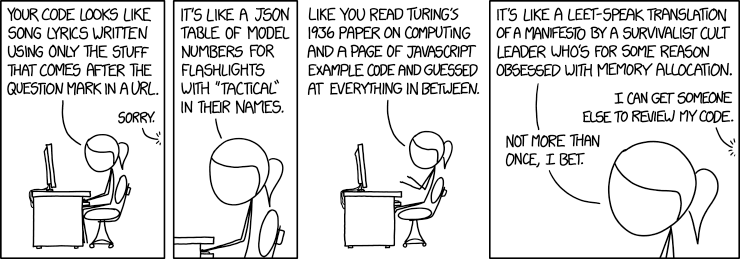
\includegraphics[width=.8\linewidth]{./gfx/17-xkcd-code_quality_3}

\vspace{12pt}
\emph{It's like a half-solved cryptogram where the solution is a piece of FORTH code written by someone who doesn't know FORTH.}

\vspace{6pt}
Source: \url{https://xkcd.com/1833/}
\end{center}
%
\end{frame}

% =========================================================================== %

\begin{frame}{Scope For Today}
%
\begin{itemize}
\item SOLID Principles
	\begin{itemize}
	\color{gray}
	\item Single Responsibility Principle
	\item Open/Closed Principle
	\color{black}
	\item Liskov Substitution Principle
	\item Interface Segregation Principle
	\item Dependency Injection Principle
	\end{itemize}
\item More Design Patterns
	\begin{itemize}
	\item Builder and Factory
	\item Observer/Listener/Subscriber
	\item Adapter
	\item Proxy
	\end{itemize}
\end{itemize}
%
\end{frame}

% =========================================================================== %

\begin{frame}{Liskov Substitution Principle}
%
\vspace{-5pt}
\begin{defbox}[Definition]
\small
Objects of a superclass should be replaceable with objects of its subclasses without breaking the application.

\vspace{-12pt}
\begin{flushright}
Barbara Liskov
\end{flushright}
\end{defbox}
\pause

\vspace{-9pt}
\begin{defbox}[Another Wording]
\small
If it Looks Like a Duck, Quacks Like a Duck, But Needs Batteries - You Have the Wrong Abstraction

\vspace{-12pt}
\begin{flushright}
Derick Bailey
\end{flushright}
\end{defbox}
\pause

\vspace{-5pt}
\begin{itemize}
\item Functions should work the same when being passed a base instance or a derived instance
\item Note that this is more a \emph{semantic} requirement rather than a \emph{syntactic} one
\end{itemize}
%
\end{frame}

% =========================================================================== %

\begin{frame}[fragile]
%
\begin{hintbox}[Syntax vs. Semantics]
\footnotesize
\emph{Syntactic requirement} refers to the rules that define what can be evaluated at all. \\
For example, given:
\begin{codebox}
\begin{minted}{python3}
def f(x, y):
    return x + y
\end{minted}
\end{codebox}
we find the syntactic requirement that \texttt{x} and \texttt{y} must be such that the addition is defined between them.
A compiler can determine syntactic correctness.

\vspace{6pt}
\emph{Syntactic requirement}, on the other hand, refers to a notion of meaning for humans. For example:
\begin{codebox}
\begin{minted}{python3}
print("Total track length:", f(x, y), "km")
\end{minted}
\end{codebox}
can be compiled with \inPy{str}ings \texttt{x} and \texttt{y}, but only \emph{makes sense} with numbers.
\end{hintbox}
%
\end{frame}

% =========================================================================== %

\begin{frame}{How This Could Even Go Wrong}
%
\begin{itemize}
\item Semantics broken in derived class
	\begin{itemize}
	\item Have a base class \texttt{B} with a method \texttt{m}
	\item Have a derived class \texttt{D}, overriding \texttt{m}
	\item Have a function \texttt{f(x : B)} that calls \texttt{m}
	\item If \texttt{D.m} does not have the same semantics as \texttt{B.m}, the LSP is not satisfied
	\item[\Thus] Take care when overriding methods
		\begin{itemize}
		\item Guideline: always call \texttt{super().m(*args, **kwargs)} in your derived methods!
		\end{itemize}
	\item[\Thus] Take care when redefining attributes
		\begin{itemize}
		\item Don't redefine attributes
		\item Guideline: use name mangling (\texttt{\_\_attribute}) when you need to re-use a name
		\end{itemize}
	\end{itemize}
	\pause
\item Semantics broken in called function
	\begin{itemize}
	\item Function \texttt{f} makes too narrow checks
	\item E.\;g. \inPy{if type(arg) != B: ...} when checking compatiblity
	\item Better: \inPy{if not isinstance (arg, B): ...} 
	\item Similar: \inPy{if not issubclass (cls, B): ...} 
	\end{itemize}
\end{itemize}
%
\end{frame}

% =========================================================================== %

\begin{frame}{By Extension: Function Signatures}
%
\begin{itemize}
\item You might write a number of functions with similar semantics
	\begin{itemize}
	\item Example Gnuplot Interface: \texttt{writeScript}, \texttt{writeScriptHead}, \texttt{writeScriptFooter}, ...
	\end{itemize}
\item Try to keep the signature (= number and type of arguments) consistent across these functions
	\begin{itemize}
	\item This may not always be possible
	\item Example Gnuplot Interface: \texttt{writeScript(fileStream)}, \texttt{writeScriptHead(fileStream)}, \texttt{writeScriptFooter(fileStream, {\color{red}pageNumber})}
	\item If the functions are methods: additional attributes can be instance attributes
	\end{itemize}
\end{itemize}
%
\end{frame}

% =========================================================================== %

\begin{frame}{Interface Segregation Principle}
%
\begin{defbox}[Definition]
\small
No code should be forced to depend on methods it does not use.
\end{defbox}
%
\begin{itemize}
\item Mostly a problem of statically typed languages
	\begin{itemize}
	\item Function \texttt{f} may expect \texttt{arg} of type \texttt{ClassWithManyMethods} ...
	\item ... but actually only uses a small subset of its methods
	\end{itemize}
\item Python: duck typed
	\begin{itemize}
	\item You can always pass \inPy{object}s
	\item Everything is an \inPy{object}
	\end{itemize}
\item Still applies, kinda
	\begin{itemize}
	\item Type hints 
	\item Explicit type checks (\inPy{if isinstance(arg, Class): ...})
	\item Abstract Base Classes
	\end{itemize}
\end{itemize}
%
\end{frame}

% =========================================================================== %\\

\begin{frame}{Example ATM}
%
\begin{columns}
\column{.4\linewidth}
\begin{itemize}
\item ATM UI: needs to accomodate different handicaps
	\begin{itemize}
	\item Most people: regular Screen
	\item Blind people: Braille Interface
	\item Alternative: Speech Interface
	\end{itemize}
\item Transactions themselves
	\begin{itemize}
	\item Modelled as separate classes
	\item Take parameters of type \texttt{ATM\_UI}
	\item[\Thus] Forces full set of UI implementations, even though only one or two are needed per \texttt{Transaction}
	\item \enquote{Fat Interface}
	\end{itemize}
\end{itemize}
%
\column{.5\linewidth}
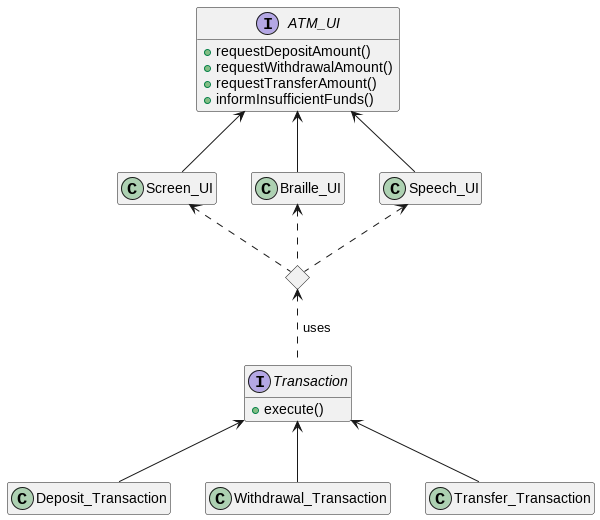
\includegraphics[width=\linewidth]{./gfx/17-uml-atm-isp_violation}
\end{columns}
%
\end{frame}

% =========================================================================== %

\begin{frame}{Why This Is A Problem}
%
\begin{itemize}
\item Valid Point: There must be an UI for all Transactions anyway, so what's the problem?
\pause
\item Remember: Changes propagate
\item A change in \texttt{Deposit\_Transaction} will require a change in \texttt{ATM\_UI}
\item This in turn might affect \texttt{Withdrawal\_Transaction} and \texttt{Transfer\_Transaction}
\pause
\item May force implementation of dummy methods
\item Example Gnuplot-Interface
	\begin{itemize}
	\item Interface \texttt{Sheet} forces existence of method \texttt{addPlotData} ...
	\item ... but there's also \texttt{MultiplotSheet} (which contains other \texttt{Sheet}s as children and cannot directly render data)
	\end{itemize}
\pause
\item Linked Languages (\zB C): Changes to a dependency often force re-compiling, which may take considerable time
\end{itemize}
%
\end{frame}

% =========================================================================== %

\begin{frame}{Solutions}
%
\begin{columns}
\column{.5\linewidth}
\begin{itemize}
\item Break up interfaces (= abstract base classes in Python) into atoms
	\begin{itemize}
	\item An interface with only one method is perfectly fine!
	\item Most often: 2..5 methods belonging to one domain
	\end{itemize}
\item Interfaces can be composed by multiple inheritance, where the need arises
\end{itemize}
%
\column{.5\linewidth}
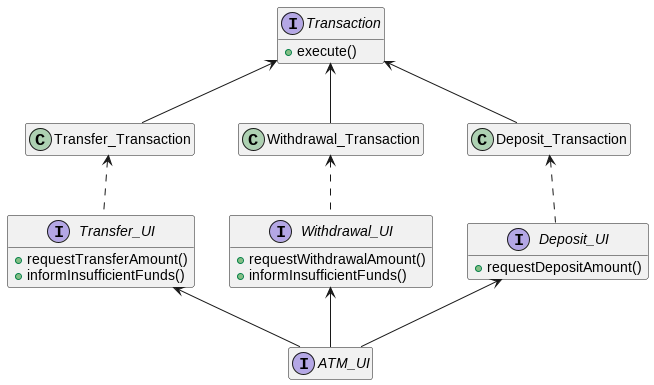
\includegraphics[width=\linewidth]{./gfx/17-uml-atm-isp_applied}
\end{columns}
%
\end{frame}

% =========================================================================== %

\begin{frame}{Tangent: Interfaces, Abstract Classes, Concrete Classes}
%
\begin{itemize}
\item Python only knows concrete classes and abstract base classes
\item Interfaces are a Java concept that doesn't really exist in other languages
\item Idea: separate abstract idea (\thus interface) from implementation (abstract/concrete classes)
	\begin{itemize}
	\item Abstract idea: Door, can be open or closed
	\item Implementation: wooden door, glass door, ...
	\end{itemize}
\item Personally, ...
	\begin{itemize}
	\item I call a class that only specifies abstract methods and no attributes an interface
	\item Abstract base classes have at least one concrete method ...
	\item ... but sometimes I still call them interfaces (\enquote{with a default implementation})
	\item Anything with attributes is an ABC (or a concrete class)
	\item Distinction in whether they belong to a particular implementation or to the abstract concept modelled by the interface
	\item[\Thus] An ABC may inherit from an interface, but not the other way round
	\end{itemize}
\item All of this: only semantics -- you may treat the terms ABC and interface as synonyms
\end{itemize}
%
\end{frame}

% =========================================================================== %

\begin{frame}{Dependency Injection Principle}
%
\vspace{-6pt}
\begin{defbox}[Definition]
\small
High-level modules should not depend on low-level modules.\\
Both should depend on abstractions.

\vspace{3pt}
Abstractions should not depend upon details.\\
Details should depend upon abstractions.
\end{defbox}
%
\vspace{-6pt}
\begin{itemize}
\item Abstraction usually means interface
\item High- and Low-Level refer ...
	\begin{itemize}
	\item ... to compositions
		\begin{itemize}
		\item Contained entities (\zB \texttt{Weapon}s like \texttt{Sword}, \texttt{Club}, ...) are low level
		\item Containing entities (\zB \texttt{Warrior}, \texttt{Ghoul}, ...) are high level
		\end{itemize}
	\item ... to a \emph{is used by} relation (Server/Client)
		\begin{itemize}
		\item Client: Entity that calls another entity
		\item Server: Entity that is called, that provides a service
		\end{itemize}
	\end{itemize}
\item[\Thus] Both, high and low end entities should be exchangeable
\end{itemize}
%
\end{frame}

% =========================================================================== %

\begin{frame}{Why the DIP is Important}
%
Dependencies are transitive!
\begin{itemize}
\item Assume you have three different layers of code: \emph{Policy Layer}, \emph{Mechanism Layer} and \texttt{Utility Layer}
	\begin{itemize}
	\item The \emph{policy layer} sets the rough state of the prorgram: show menu, validate inputs, produce outputs, ...
	\item The \emph{mechanism layer} defines what these states mean: shape of user interface, validation criteria, ...
	\item The \emph{utility layer} provides the tools with which the \emph{mechanisms} are implemented: \texttt{drawButton}, \texttt{readFile}, ...
	\end{itemize}
\pause
\item Naively, one would make the \emph{policy layer} dependent on the \emph{mechanism layer}, which in turn depends on the \emph{utility layer}
\item[\Thus] Changes in the \emph{utility layer} will percolate up to the \emph{policy layer}!
\item[\Thus] Likewise when \emph{naively} inverting the direction of dependency
\end{itemize}
%
\end{frame}

% =========================================================================== %

\begin{frame}{Why the DIP is Important}
%
Dependencies imply mode of usage
\begin{itemize}
\item Think of a \texttt{CopyCreator} class/application
	\begin{itemize}
	\item Reads some input from one file
	\item Writes it into another file
	\end{itemize}
\pause
\item Abides by the SRP
	\begin{itemize}
	\item Has a \texttt{FileReader} and a \texttt{FileWriter} class
	\item[\Thus] The CTor of \texttt{CopyCreator} instantiates one \texttt{FileReader} and one \texttt{FileWriter}
	\end{itemize}
\item[\Thus] Your higher level \texttt{CopyCreator} depends on the lower level \texttt{FileReader} and \texttt{FileWriter}
\pause
\item Now, you might later come up with a \texttt{NetworkStreamReader} ...
\item ... or a \texttt{ToScreenWriter}
\item[\Thus] The top-down dependency structure prevents extensibility!
\end{itemize}
%
\end{frame}

% =========================================================================== %

\begin{frame}{Solution}
%
\vspace{-9pt}
\begin{columns}
\column{.35\linewidth}
\begin{center}
\small
conventional structure\\
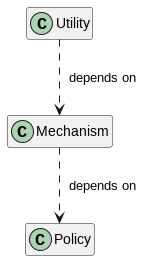
\includegraphics[width=.3\linewidth]{./gfx/17-uml-dependency_injection-violation}

\vspace{6pt}
inverted structure\\
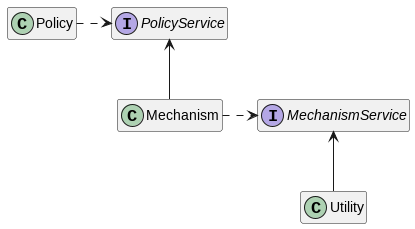
\includegraphics[width=\linewidth]{./gfx/17-uml-dependency_injection-applied}
\end{center}
%
\column{.6\linewidth}
\begin{itemize}
\item Insert interfaces (abstractions) between entities
	\begin{itemize}
	\item Not only dependeny inversion ...
	\item ... but separation!
	\end{itemize}
\item Lower levels implement interfaces
	\begin{itemize}
	\item[\Thus] Do not know who uses them ...
	\item[\Thus] ... but know they are used in intended way
	\end{itemize}
\item Higher levels expect interfaces
	\begin{itemize}
	\item[\Thus] Not bound to a particular implementation ...
	\item[\Thus] ... but to a \emph{reasonable} entity
	\end{itemize}
\item Inversion
	\begin{itemize}
	\item of dependency direction (of concrete implementations)
	\item of ownership (interfaces belong to one level up)
	\end{itemize}
\end{itemize}
\end{columns}
%
\end{frame}

% =========================================================================== %

\begin{frame}{Corrolary: Constructor Arguments}
%
\begin{itemize}
\item Traditional approach: initialize components in the CTor
	\begin{itemize}
	\item \inPy{self.component = ComponentClass()}
	\end{itemize}
\pause
\item If high level entity can only depend on abstractions, this is no longer possible
	\begin{itemize}
	\item Abstraction is an interface, \ie an abstract base class
	\item Cannot be instantiated
	\end{itemize}
\pause
\item[\Thus] Injection part of Dependency Injection Principle
	\begin{itemize}
	\item Pass the actual, concrete component as a parameter
	\item Signature of CTor only demands an ABC
	\item[\Thus] \inPy{def __init__(self, component: ComponentInterface)}
	\end{itemize}
\pause
\item Possibly requires a problematic number of arguments
	\begin{itemize}
	\item Many arguments \Thus many chances to forget, mix up order or otherwise make errors
	\item Mitigation: Python allows keyword arguments
	\item[\Thus] \inPy{instance = CompositeObject(component = ComponentClass(), ...)}
	\end{itemize}
\end{itemize}
%
\end{frame}

% =========================================================================== %

\begin{frame}{Alternative to Constructor Arguments}
%
\begin{itemize}
\item Alternative
	\begin{itemize}
	\item Initialize to \inPy{None}
	\item Inject via Setter method
	\end{itemize}
\pause
\item Advantages
	\begin{itemize}
	\item Easy to implement, easy to use, easy to understand
	\end{itemize}
\pause
\item Disadvantages
	\begin{itemize}
	\item Easy to forget calling a setter
	\item[\Thus] Possibly invalid state of an entity
		\begin{itemize}
		\item Example: Rogue Like, construct \texttt{Enemy}: Forget to call \texttt{setWeapon}
		\item Attack Phase contains \inPy{weapon.getDamage()}
		\item[\Thus] Crash (\texttt{NoneType} does not have method \texttt{getDamage})
		\end{itemize}
\pause
	\item Forcibly makes entity mutable
	\item[\Thus] Harder to guarantee validity of entity throughout its lifecycle
		\begin{itemize}
		\item E.\;g. Enemy with two-handed weapon \emph{and} shield
		\end{itemize}
	\end{itemize}
\pause
\item Solution: Builder Pattern
\end{itemize}
%
\end{frame}

% =========================================================================== %

\begin{frame}[fragile]{Builder Pattern}
%
\vspace{-3pt}
\begin{itemize}
\item Solution: Builder class for each Enemy
	\begin{itemize}
	\item \texttt{GhoulBuilder}, \texttt{TrollBuilder}, etc.
	\item Separate class that collects all the items one by one
		\begin{itemize}
		\item Has a setter for each needed characteristic
		\end{itemize}
	\item Has a \texttt{build} method that returns the \texttt{Enemy}
		\begin{itemize}
		\item Passes characteristics on to the \texttt{Enemy} CTor
		\end{itemize}
	\item Optionally: \texttt{build} performs validity check 
		\begin{itemize}
		\item \texttt{Ghoul} not allowed to have a \texttt{Bow}
		\item Forgot to set \texttt{underwearColour}
		\end{itemize}
	\end{itemize}
\pause
\item Advantages
	\begin{itemize}
	\item Preserves ease of use of the setters approach
	\item Maintains immutability
	\item Guarantees validity of entity
	\end{itemize}
\pause
\item Disadvantage
	\begin{itemize}
	\item Two coupled classes
	\item Not immediately clear that Builder should be used
		\begin{itemize}
		\item Other languages often: \emph{private friended CTor}
		\end{itemize}
	\end{itemize}
\end{itemize}
%
\end{frame}

% =========================================================================== %

\begin{frame}{Related: Factory Pattern}
%
\begin{itemize}
\item Game should be procedurally generated
	\begin{itemize}
	\item[\Thus] Program decides which and how many enemies appear
	\end{itemize}
\item Should be consistent with environment
	\begin{itemize}
	\item E.\;g. encounter trolls only in mountains, ghouls in catacombs, warriors everywhere
	\end{itemize}
\item[\Thus] Need a mechanic for \emph{environment state} \thus \emph{enemy constructor/builder}
	\pause
\item Solution: Factory
	\begin{itemize}
	\item Class that takes some context values (\zB landscape ID) 
	\item Returns appropriate class instance (\zB random \texttt{EnemyBuilder} for that region)
	\item Subtle difference between Factory and Builder
\pause
	\item For simple cases, a Factory can also be a Builder ... 
	\item but this violates the SRP!
	\end{itemize}
\end{itemize}
%
\end{frame}

% =========================================================================== %\\

\begin{frame}
%
\begin{center}
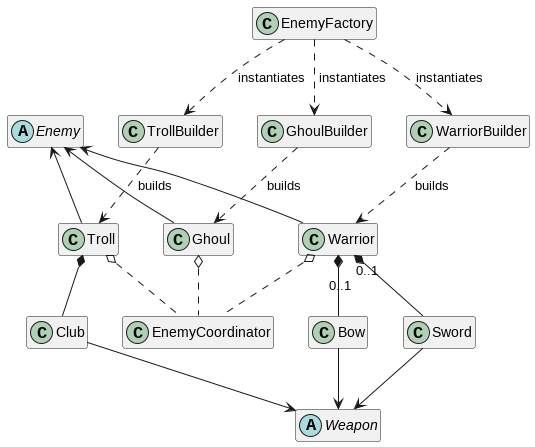
\includegraphics[width=.65\linewidth]{./gfx/15-uml-big}
\end{center}
%
\end{frame}

% =========================================================================== %

\begin{frame}{Observer Pattern (aka Listener Pattern, aka Subscriber Pattern)}
%
\begin{itemize}
\item Class \texttt{EnemyCoordinator}
	\begin{itemize}
	\item \enquote{Makes decisions for instances of} \texttt{Enemy}
	\item Whom to attack, where to move, ...
	\item Might also decide: do nothing
	\end{itemize}
\item[\Thus] Needs to know whom to coordinate
\item[\Thus] Needs to communicate with its \emph{clients}
\pause
\item[\Thus] Establish communication protocol
	\begin{itemize}
	\item \texttt{EnemyCoordinator} has \texttt{addSubscriber(s : Subscriber)}
		\begin{itemize}
		\item Internally: add to \inPy{list} of \texttt{Subscriber}s
		\end{itemize}
	\item Every \texttt{Subscriber} has method \texttt{listen(i : Instruction)}
	\item \texttt{EnemyCoordinator} has method \texttt{broadcast()}
		\begin{itemize}
		\item Calls \texttt{s.listen(i)} for each \texttt{Subscriber}
		\end{itemize}
	\end{itemize}
\end{itemize}
%
\end{frame}

% =========================================================================== %

\begin{frame}{Adapter Pattern}
%
\begin{itemize}
\item Discussed coding style imposes a lot of formal requirements
	\begin{itemize}
	\item Must be subtype of a given class
	\item Must satisfy a certain interface
	\end{itemize}
\pause
\item Sometimes: entities logically capable of a desired operation, but form not satisfied
	\begin{itemize}
	\item Wrong parent class(es)
	\item Wrong return type of a method
	\end{itemize}
\item Inconvenient or impossbile to make changes
	\begin{itemize}
	\item OCP violation
	\item Third party library
	\item ISP violation: fat interfaces
	\end{itemize}
\pause
\item Adapter class
	\begin{itemize}
	\item Wrapper around the entity
	\item Satisfies formal requirements
	\item Internally calls the actually provided methods and/or makes conversions
	\end{itemize}
\end{itemize}
%
\end{frame}

% =========================================================================== %

\begin{frame}{Proxy Pattern}
%
\begin{itemize}
\item Also: Wrapper around concrete object
\item Aim: Access Control
\item Example: Database Connection
	\begin{itemize}
	\item Expensive to set up, not always needed
	\item Desired: Lazy initialization, Singleton pattern
	\end{itemize}
\item Limitations / Reasons for the Pattern
	\begin{itemize}
	\item OCP or even third party tool
	\item DRY: deferred (lazy) initialization requires special setup
	\end{itemize}
\item[\Thus] Proxy object handles all of this, clients use Proxy instead
\end{itemize}
%
\end{frame}

% =========================================================================== %

\begin{frame}{More Patterns, More Literature}
%
\begin{itemize}
\item See \url{https://refactoring.guru/design-patterns}
\item We've already covered some of them before today
	\begin{itemize}
	\item Decorator (see lecture 2)
	\item Iterator (see lecture 3)
	\item Singleton (see lecture 13)
	\end{itemize}
\item More Literature
	\begin{itemize}
	\item Robert C. Martin Series
		\begin{itemize}
		\item Clean Code
		\item Agile Principles, Patterns, and Practices in C\#
		\end{itemize}
	\end{itemize}
\end{itemize}
%
\end{frame}

% =========================================================================== %

\begin{frame}{Conclusion}
%
\begin{itemize}
\item Proper encapsulation solves a lot of problems
\item SRP, OCP, LSP, ISP, DIP all boil down to encapsulation / KISS
	\begin{itemize}
	\item Seem to add complexity ...
	\item ... but that complexity was always there
	\item Breaks it down to bite sized chunks ...
	\item ... and exposes the true complexity of the problem at hand
	\end{itemize}
\item Implementing this encapsulation takes some upfront effort ...
\item ... but it's well worth it once projects grow beyond a certain complexity
\pause
\item The SOLID principles are particularly prevalent in the Java ecosphere,
	\begin{itemize}
	\item which is (partially) the reason why Java is said to be 99\% boiler plate code ...
	\item ... but the language is still heavily used in professional context, probably exactly because of adapting these scalability principles
	\end{itemize}
\end{itemize}
%
\end{frame}

% =========================================================================== %

\begin{frame}
%
\begin{center}
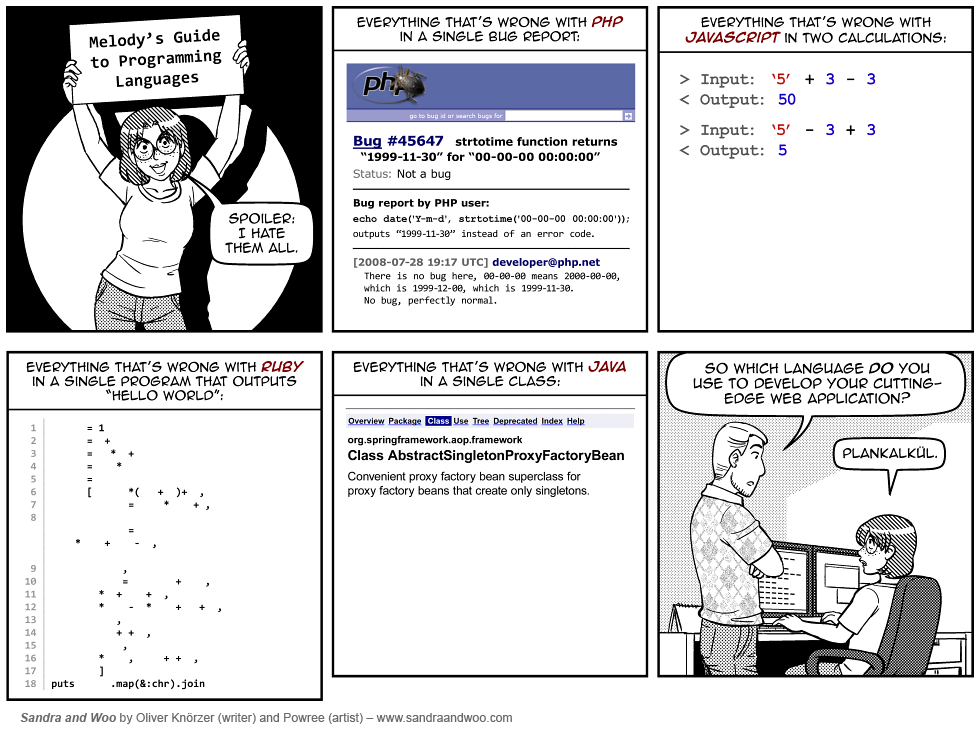
\includegraphics[width=.75\linewidth]{./gfx/17-saw-melodys-guide-to-programming-languages}

\tiny
\url{http://www.sandraandwoo.com/2015/12/24/0747-melodys-guide-to-programming-languages/}
\end{center}
%
\end{frame}

% =========================================================================== %

\end{document}

% MAREI!!
% whom do I give credit? Where?